\documentclass[journal]{./IEEE/IEEEtran}
\usepackage{cite,graphicx}
\usepackage{url}

\newcommand{\SPTITLE}{QRSMS: SMS client with end-to-end encryption via Quick Response (QR) code}
\newcommand{\ADVISEE}{John Mel R. Ramos}
\newcommand{\ADVISER}{Jaderick P. Pabico}

\newcommand{\BSCS}{Bachelor of Science in Computer Science}
\newcommand{\ICS}{Institute of Computer Science}
\newcommand{\UPLB}{University of the Philippines Los Ba\~{n}os}
\newcommand{\REMARK}{\thanks{Presented to the Faculty of the \ICS, \UPLB\
		in partial fulfillment of the requirements
		for the Degree of \BSCS}}
\markboth{CMSC 190 Special Problem, \ICS}{}
\title{\SPTITLE}
\author{\ADVISEE~and~\ADVISER%
	\REMARK
}
\pubid{\copyright~2006~ICS \UPLB}
%%%%%%%%%%%%%%%%%%%%%%%%%%%%%%%%%%%%%%%%%%%%%%%%%%%%%%%%%%%%%%%%%%%%%%%%%%
\begin{document}
	
% TITLE
\maketitle
	
% ABSTRACT
%\begin{abstract}
%The quick brown fox jumps over the lazy dog near the riverbank.
%\end{abstract}

% INDEX TERMS
%\begin{keywords}
%SMS, end-to-end encryption
%\end{keywords}

% OUTLINE:
% Brief history of SMS including its use cases in the current era of mobile communications
% Why is securing SMS important
% Why SMS is still relevant today.
% Explain the scope and limitations of the proposed client.
% Literature Review
% Methodology

% INTRODUCTION
\section{Introduction}
%1. Why is the problem of interest? 1-2 pars
Despite the emergence of instant messaging (IM) and Over-the-top (OTT) 
messaging applications, short message service (SMS) remains as a popular option 
for mobile communication. With the first text message sent in 1992 through the 
Global System for Mobile communication (GSM) network, the technology has seen 
a lot of growth and  development~\cite{LeBodic_2005}. While mostly used for 
person-to-person communication \cite{Herring_Stein_Virtanen_2013}, the medium 
has seen other applications such as alert notification~\cite{Yoo_Lee_Yoo_Xiao_2021,
Azid_Sharma_Raghuwaiya_Chand_Prasad_Jacquier_2015}, 
empowering businesses and online services~\cite{Gargaro_2023, Okazaki_Taylor_2008, 
SecureSMS14}, mobile health (m-health) interventions~\cite{NudgeFlu23, SMSUx22}, 
mobile government applications~\cite{Onashoga_Ogunjobi_Ibharalu_Lawal_2016, EGov13},
education~\cite{Hill_Hill_Sherman_2007}, Two-Factor Authentication (2FA)
~\cite{DynamicOTP} and more. During the year 2022, Globe Telecom gained 
Php 8.8 billion revenue from SMS with 86.7 million mobile customers. 
Furthermore, the company has invested Php 1.1 billion to improve spam and 
fraudulent SMS detection and prevention~\cite{GlobeIR22}. Unreliable internet 
service as well as the lack of Internet infrastructure in some area remains a 
challenge in the adoption of online services for communication such as 
Facebook Messenger, Viber, Telegram, etc. SMS on the other hand is ubiquitous. 
Anyone with a mobile device and a registered subscriber identity module (SIM) 
card can send and receive text messages regardless of their platform and 
cellular provider~\cite{PhilStar}. 

Regardless of its wide range of applications and sustained use, however, 
SMS is not ideal for private communication such as sending sensitive and 
confidential information as early specifications for SMS does not have security 
in mind~\cite{3gpp2}. The European Telecommunications Standards Institute (ETSI) 
specified the use of A5 algorithm for encryption over the GSM network together 
with the A3 and A8 algorithm for authentication and cipher key generation to 
provide security~\cite{Schiller2011} but attacks on the A5/1 and the weaker 
A5/2 algorithms has been demonstrated even with minimal resources
~\cite{a512001, a522007,Barkan_Biham_Keller_2003} and even the A5/3 used for 
Third Generation (3G) network has been compromised~\cite{a532010}. 
Mobile network operators may also opt not to use any encryption during the 
transit of message wirelessly~\cite{gsm348}. This means that a 
Man-in-the-Middle (MITM) can sit between the Mobile Equipment (ME) and 
Base Station Subsystem (BSS) using an International Mobile Subscriber Identity 
(IMSI) catcher to actively intercept traffic and even request the victim ME 
to use a weaker or no encryption at all~\cite{Cattaneo_DeMaio_Faruolo_Petrillo_2013}. 
Additionally, encryption is only performed between the Mobile Equipment (ME) 
and the Base Station Subsystem (BSS)~\cite{Schiller2011}. Once the message 
reaches the SMS Center (SMSC), messages are stored and kept in plain text for a 
while allowing malicious entities to target the SMSC to 
view the contents of these messages. This makes an end-to-end encryption a huge
improvement over what is available in the GSM specifications.

%2. What is the background of the solutions proposed by others? (summary of literature review, 1 par)
To provide a better security system for SMS, independent researchers have
proposed frameworks and protocols that offers end-to-end encryption.
PK-SIM~\cite{PKSIMcard07} provides end-to-end security between the mobile user 
and service provider through Public Key Infrastructure (PKI).
SMSSec~\cite{SMSSec08} was developed using the Java Wireless Messaging API (WAP)
and uses a combination of asymmetric and symmetric cryptography to provide
security. EasySMS~\cite{EasySMS14} and SecureSMS~\cite{SecureSMS14} are
completely based on symmetric key cryptography. Similarly, SmartSMS
~\cite{SmartSMS16} uses symmetric key encryption for m-health application.
These protocols however, requires additional resources and infrastructure
on the side of the service provider in order to be implemented.

%3. What is the background of my proposed solution? (rev of my solution), 1 par
In this paper, we propose an SMS client that uses 
quick-response (QR) codes for key exchange. Initially developed by Toyota's
subsidiary Denso Wave for inventory of vehicle parts manufacturing,
QR code has seen many application in today's era~\cite{Tiwari_2016}.
Able to store up to a maximum of 7,089 characters in one code~\cite{qrcode}
it can be used to encode text, URL, and other data and can be decoded using
a mobile device equipped with a camera and the appropriate software which can
display a text, connect to a wireless network, open a webpage, or open a linked
application~\cite{Shin_Jung_Chang_2012}. The proposed client will encode the
public key and parameters needed to generate a shared secret in a QR code. The
code can be shared to the intended recipient through offline (in person)
or other secure online platform that allows sending of images.

End-to-end security will be achieved through the combined use of symmetric and
asymmetric cryptography as well a key-agreement protocol. Advaned Encryption
Standard (AES) will be used for encrypting the message as it provides the
most security while being performant~\cite{Karale_Pendke_Dahiwale_2015}.
Elliptic Curve Cryptography (ECC) will be used for generating key pairs and
Elliptic Curve Diffie-Hellman (ECDH) for generating a shared secret. The use
of ECC allows for a smaller key length while providing an comparable security
as the Rivest–Shamir–Adleman (RSA) public key cryptosystem~\cite{Amara_Siad_2011}.

%4. What will I do? (summary of my methodology), 1-2 par
Using the android platform, we will develop an SMS client that can generate
keypair, exchange public keys through QR code, and establish an end-to-end
encrypted communication. 

%5. What do I expect to happen?

% REVIEW OF RELATED LITERATURE
\section{Literature Review}
PK-SIM \cite{PKSIMcard07} card based framework  was proposed to 
provide end-to-end encryption. 
Taking advantage of the tamper resistant properties of the Subscriber Identity Module (SIM) card inside  mobile phones to store and protect secrets, the PK-SIM card is a standard SIM equipped with PKI functionality.
The SMSSec \cite{SMSSec08} protocol uses the Java Wireless Messaging API (WAP) to secure SMS communication.
It uses asymmetric cryptography once for the first hand-shake to establish a secure channel for communication and a symmetric cryptography on the succeeding exchanges due to its lesser computational cost. In contrast, the EasySMS \cite{EasySMS14} protocol is designed to provide end-to-end encryption using only symmetric algorithm. 
These protocols rely on an authentication server or a certificate authority to validate the indentities of the involved mobile systems to establish a secure communication channel. 
Using the same concept from EasySMS, SecureSMS \cite{SecureSMS14} is made for Value Added Services (VAS) applications. Authors found their protocol to be 71\% and 59\% more efficient than the PK-SIM and SMSsec in terms of bandwidth for authentication. 
SmartSMS \cite{SmartSMS16} protocol is developed for secure m-health environment application. This protocol relies on an authentication server (AS) to generate the shared session key between the sender and receiver and a Trusted Third Party hosted in the cloud to validate the identities of the mobile station.  

% \section{Objectives}
% 1 General Objective - 1 sentence
% At least 3 specific objective to support the primary objective
\section{Objectives}
% In this section you state what you want to accomplish. First state the 
% general objective then the specific objectives. Your results after the 
% implementation should achieve the objectives you stated.
To provide a secure platform for the exchange of encrypted SMS, the main
objective of this research is to develop an SMS client application that
can encrypt and decrypt messages and utilize QR codes as means of
exchanging keys for generating a shared secret. To be specific, this research
aims to do the following:
\begin{itemize}
    \item[1.] Implement a keypair generator and encode the public key on a
        QR code.
    \item[2.] Implement a decoder to retrieve the keys in the QR code and
        generate a shared secret using a key-agreement protocol.
    \item[3.] Implement an SMS client with cryptographic capabilities
        using the android system's built in libraries.
\end{itemize}


% The Methodology section should describe the approach you are going to 
% take to solve the problem. You can use the software development lifecycle 
% as an outline: Requirements, Design, Implementation, and Testing.
% A timeline is also required in this section. You can use a Gantt chart 
% for this at least at the week level granularity. At the proposal stage, 
% you should write the methodology in future tense.
\section{Materials and Methods}
Equipped with features and support for developing android applications,
Android Studio will be used as the integrated development environment (IDE).
The programming language Kotlin will also be used for the application as it
eliminates the verbosity of Java while also allowing the use of Java libraries
~\cite{Moskala_Wojda_2017}. The android platform comes with telephony and 
cryptographic libraries that will help achieve the goals of the 
application~\cite{android_pkg}.

\subsection{Requirements}
In order to achieve the main purpose of this application, the following
requirements must be considered. The application should be able to:
\begin{itemize}
    \item[1.] Send and receive encrypted SMS message.
    \item[2.] Decrypt encrypted SMS message.
    \item[3.] Generate a private and public key pair.
    \item[4.] Encode the user's public key along with other parameters
        needed to perform a key exchange into a QR code.
    \item[5.] Decode the QR code containing the other participant's public
        key and parameters to generate the shared secret.
    \item[6.] Safely store secrets inside the device.
    \item[7.] Associate the correct keys to the appropriate contact.
    \item[8.] Allow users to manage saved keys.
\end{itemize}

It should also be noted that in order to keep the integrity of the system,
we have to make the assumption that the user will not feed a QR code
whose origin is unknown. To ensure that the code being decoded is from the 
intended contact, it goes without saying that the QR code should only come
from the other party involved in the secure communication. 
While there will be verification if the encoded data
are valid, this assumption will help protect the user against adversaries.

\subsection{System Design}
To achieve end-to-end encryption, the application can be broken into three
major steps --- keypair generation, key-agreement protocol, and
encrypted messaging.
\begin{figure*}
    \centering
    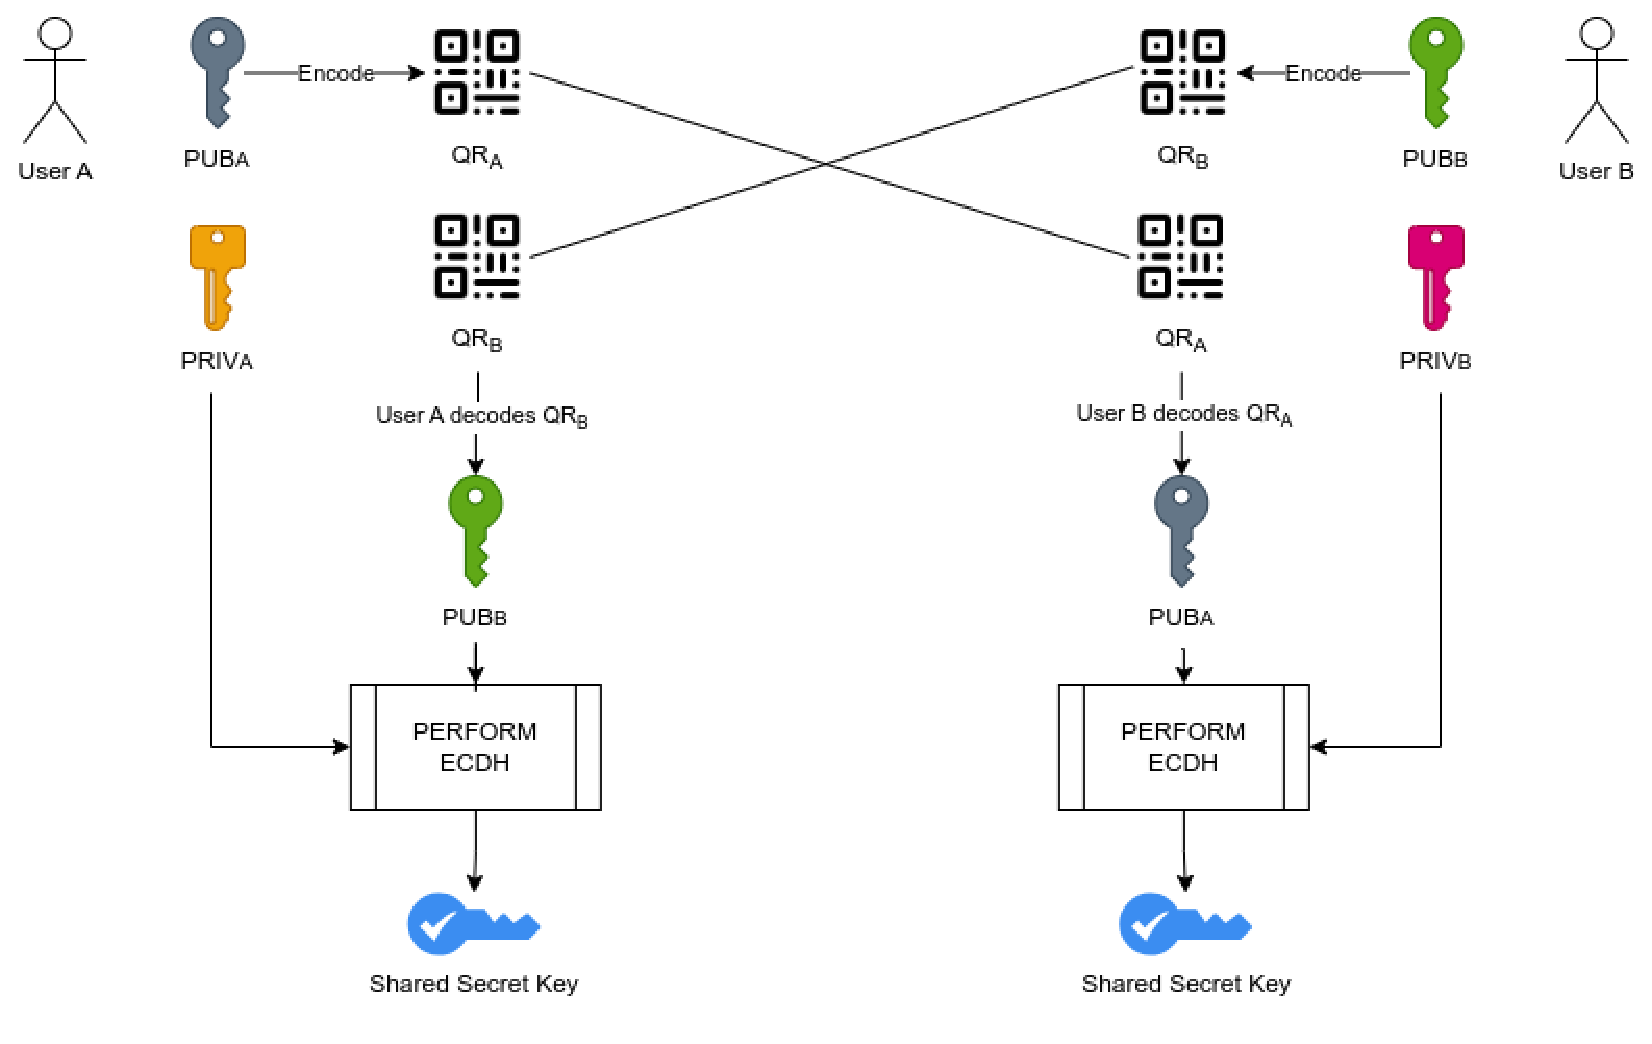
\includegraphics[width=6in]{images/key_agreement.eps}
    \caption{Overview of key generation and key agreement in QRSMS}
    \label{key_genagree}
\end{figure*}

\subsubsection{Keypair Generation}
Before enabling the exchange of encrypted messages, each party involved
must first generated their public and private key pair. For each contact the
user wants to exchange keys with, a unique key pair will be generated.
We will be using Elliptic Curve (EC) algorithm for the generation.
The generated public key will be encoded to a QR code while the complementing
private key will be kept securely in the system and will be used to finalize
the key exchange.

\subsubsection{Key-Agreement Protocol}
Once each party have their generated QR code, they will give their QR code to
the other allowing them to scan and use the key. Using ECDH, their private key
for that particular user will be fed along with the scanned public key to
generate a shared secret. The shared secret will be stored inside Android's
built in KeyStore to protect the keys from unauthorized use~\cite{android_keystore}.

\begin{figure*}
    \centering
    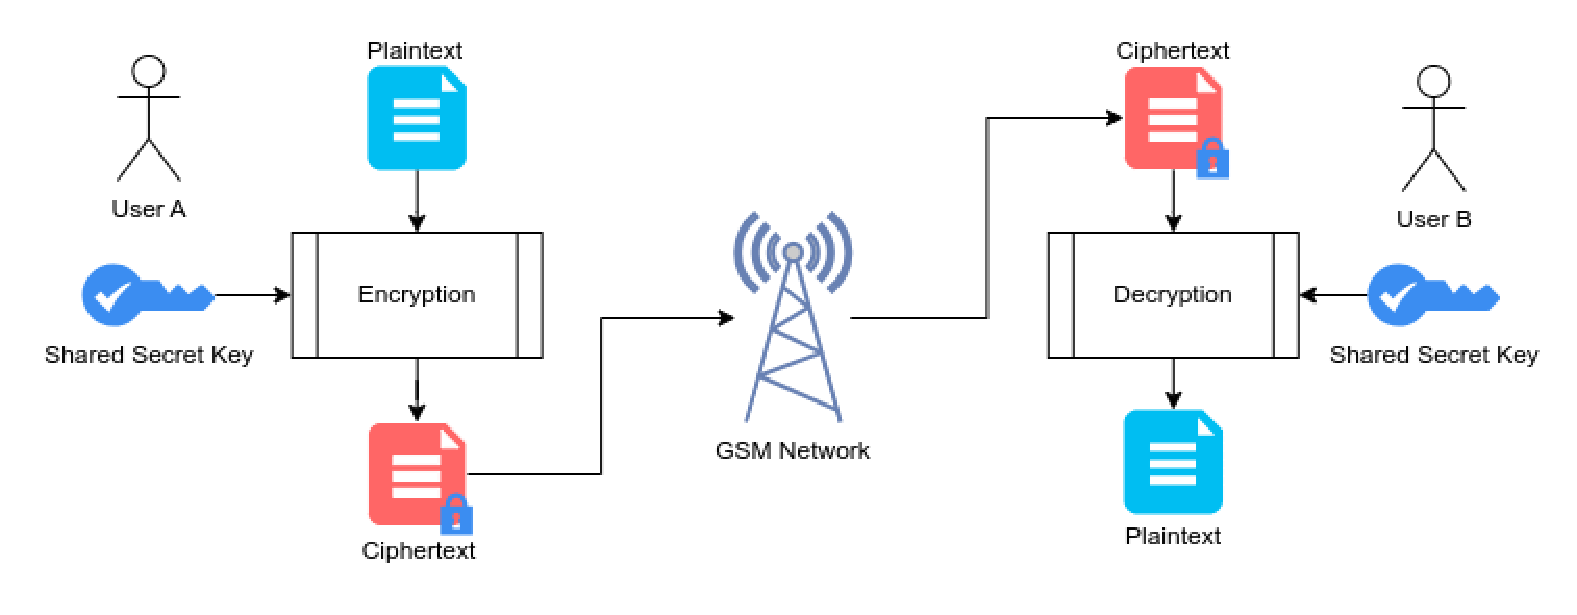
\includegraphics[width=6in]{images/encrypted_messaging.eps}
    \caption{Overview of sending and decryption of messages in
    QRSMS}
    \label{encrypted}
\end{figure*}

\subsubsection{Encrypted Messaging}
With each of the user involved in the key-agreement now having generated a
shared secret with their intended contact, the exchange of encrypted SMS
can now begin. Using AES encryption, we can generate an encrypted ciphertext
with the shared secret as the key for symmetric cryptography. 

Fig.~\ref{key_genagree} and fig.~\ref{encrypted} shows an overview of how 
the system will work. While each of the individual step can be implemented 
individually, the order of their execution is important as the input for the 
succeeding step relies on the previous. 

The javax.crypto library contains the KeyAgreement class needed to
establish a shared secret as well as the Cipher class that contains the 
functionalities for symmetric encryption. The java.security library will
enable us to use the KeyGenerator class which allows the generation of
public and private key pair using EC. On the other hand, there is no built-in
libraries for encoding and decoding of QR code. For that, zxing~\cite{zxing}
and google's ML kit barcode scanning~\cite{mlkit} will be bundled to 
provide the missing functionalities.

% To DO:
% Find appropriate algorithm for key exchange, and encryption algorithm than does not excede 160 character per message

% How I would want to conclude:
% While this approach does not protect against the most common attacks against SMS, through the use of the app, some form of privacy could be had as long as the shared secret remains secured.

% APPENDICES
%\appendices

%\section{Proof of the First Zonklar Equation}
%Appendix one text goes here...
%
%\section{}
%Appendix two (without title) text goes here...

% ACKNOWLEDGMENT
%\section*{Acknowledgment}
%Many thanks to...
	
% BIBLIOGRAPHY
\bibliographystyle{./IEEE/IEEEtran}
\bibliography{./ramos-cs190-ieee}
% \nocite{*}

% BIOGRAPHY
%\begin{biography}[{\includegraphics{./yourPicture.eps}}]{Student M. Name}
%Biography text here...
%\end{biography}
	
\end{document}
